
\chapter{绪论}
生活中,我们观察物体、辨别物体总是遵循“光沿直线传播”、“所见即所得”的传统光学成像规律,常见的视觉成像系统像人眼、照相机以及光学成像工具如放大镜、显微镜和望远镜等都以此为物理基础。传统光学成像主要通过提取弹道光(或抑制散射光)的方式解决透过无散射(或者弱散射)介质的成像问题。当光透过生物组织、烟尘和云雾等强散射介质时,传统光学成像规律失效。其主要原因是光在强散射介质中传播时,介质中大小为波长量级的粒子对入射光波产生的散射作用使原本有序的波前相位产生严重畸变,出射光场变得随机且紊乱,最终在观测面上只能接收到散斑图案,难以实现对目标的观测或成像。因此,散射效应成为制约透过散射介质成像技术发展的瓶颈和关键问题。

近年来,随着计算机技术飞速发展、介观物理研究的深入、计算成像思想的完善和图像处理技术的发展,形成以物理机制为基础的计算光学成像技术。计算光学成像技术作为新型成像手段,不仅推动了传统成像的发展,而且在解决散射成像方面表现出了得天独厚的优势。经过各国科学家们的不懈努力,计算成像理论以及相关实验技术迅速发展,取得了许多突破性研究成果。在弹道光提取方面,如:自适应光学成像技术 (Adaptive optics technique)、门选通技术、光学相干层析 (Optical coherence tomography)、共聚焦显微 (Confocal microscopy)、多光子显微 (Multiphoton microscopy)、光声显微 (Optoacoustic microscopy) 、合荧光分子层析 (Hybrid fluorescence molecular tomography)、多光谱光声层析 (Multispectral optoacoustic tomography) 等光学成像技术的发展及应用,解决了天文成像、水下探测和生物成像等领域的关键问题。在散射光利用方面:随着空间光调制器 (Spatial light modulator,SLM)、数字微镜器件 (Digital micromirror device,DMD)、微机电系统调制器 (Micro electro mechanical system,MEMS) 等数字波前整形器件的出现,促使了计算成像技术和散射成像技术有机的结合,涌现出了许多新型光学成像技术,如:光学相位共轭 (Optical phase conjugation)、波前反馈调节 (Wavefront shaping technique)、基于光学传输矩阵 (Transmission matrix) 等,极大地促进了散射成像技术在显微成像领域的应用。与此同时,随着对光学记忆效应 (Optical memory effect) 的深入研究,散斑相关成像技术 的提出为透过散射介质成像打开了崭新的局面。随着计算光学成像的进一步发展,基于点扩散函数 (Point Spread Function, PSF) 工程 和深度学习 的方法,也成为了解决透过散射介质成像的重要途径。

纵观散射成像的发展历程,随着对散射机理研究的不断深入,散射成像技术已从早期基础理论研究到实验室下模型验证研究再到透过散射介质成像应用研究。早期的散射成像技术注重于克服散射或抑制散射,通过弹道光与散射光的分离,最终获取有效的目标信息。现阶段的散射成像技术侧重于散射光的利用,充分挖掘散射光的特性,实现从不可探测到可探测质的飞跃。值得注意的是,散射成像技术不仅在显微成像和超分辨成像方面有着广泛的应用,而且也将在全息成像、光纤成像和光通讯等领域扮演着重要的角色。

现有透过散射介质成像方法主要有波前整形和基于光学记忆效应的散射成像技术。波前整形技术,包含光学相位共轭、基于反馈优化的波前整形和光学传输矩阵技术三部分,该技术主要研究光波在介质中的传播规律以及特性,为散射效应的利用奠定基础。基于光学记忆效应的散射成像技术,包含散斑相关成像技术和点扩散函数工程成像技术两部分,该技术核心在于对于散斑能量的利用,利用的散斑分布特点实现透过散射介质成像及相关工作。本文分别对以上方法在散射成像相关成果以及进展进行归纳和总结,并对未来的发展趋势进行了分析与展望。

\section{基于波前整形的散射成像技术}

在散射介质中传播受到散射效应的影响,在像面形成系列散斑。如何定量或定性描述散射介质在光传播过程中的影响成为利用光散射效应的关键问题。虽然光在多重散射介质中传播具有很高的随机性,但当散射介质处稳定于状态时,光在散射介质中的传播具有确定性。散射介质的特性可以与多模光纤进行类比,其输出光场可看作多种模式之间的耦合与叠加。为了精确地描述散射介质在光传播过程的作用,光学传输矩阵思想被提出,有效地将入射光场和出射光场联系起来。近年来,随着光散射理论和实验技术的飞速发展,研究人员基于光学相位共轭、反馈优化的波前整形和光学传输矩阵等技术,实现了透过散射介质的聚焦或者成像。在未获得完善的光学传输矩阵的前提下,为实现透过散射介质聚焦或成像,通常采用光学相位共轭技术或者基于反馈优化的波前整形技术;在测得完备的光学矩阵之后,往往利用光学传输矩阵技术能够有效地实现对出射光场的控制。研究结果表明,波前整形技术在生物医学成像、超分辨成像和光通信等方面有着巨大的应用前景。

\subsection{光学相位共轭}

光学相位共轭技术是时间反演技术在光学领域的应用,最早的光学相位共轭技术通过在照相板上记录全息图来实现。本质上,光学相位共轭技术利用光传播的可逆性,通过获得透过介质后的光场分布,反向输入透射光场的相位共轭波形,重建原始的入射光场。光学相位共轭实现可以分为两步:第一步,光场信息的记录;第二步,相位共轭光的生成。按照相位共轭光产生方式的不同,光学相位共轭技术可以分为非线性光学相位共轭技术和数字光学相位共轭技术两类。前者可以使用数字全息或定量相位成像技术来实现,后者是空间光调制器实现。在实验中,我们通常只能获取介质一面光场信息(或者获取部分入射光和部分散射光),在多重散射材料的情况下(也在混沌腔的情况)甚至有限的相位共轭也可以地重建部分的入射光场信息。
依据非线性过程的差异,非线性光学相位共轭技术可以分为:三波混频相位共轭技术、四波混频相位共轭技术、受激布里渊散射相位共轭技术和光折变晶体相位共轭技术。总体而言,非线光学相位共轭技术实施起来比较复杂,通常需要非线性晶体、特定波长和强激光光源。虽然实施起来比较复杂,但是非线性相位共轭技术自早期以来多用于透过复杂介质聚焦。光折变晶体作为光学相位共轭技术的一种常用手段,虽然其调节速度较慢,但可实现透过厚生物组织的聚焦成像。随着材料技术的飞速发展,许多新型光学共轭材料被研发出来,其调节速度可与SLM相媲美。许多增益介质能够提供快速的光学共轭调节,但受到其物理效应的限制,仅适用于窄谱光源。三波混频相位共轭技术具有速度快频带宽的特点,但其有效角度较小。与数字光学相位共轭技术相比,非线性光学相位共轭技术在模式耦合效率方面具有较大优势,往往高出$1 \sim 2$数量级。因此非线性光学相位共轭技术在生物医学方面仍然具有很大的潜力。

\begin{figure}[htp]
	\centering
	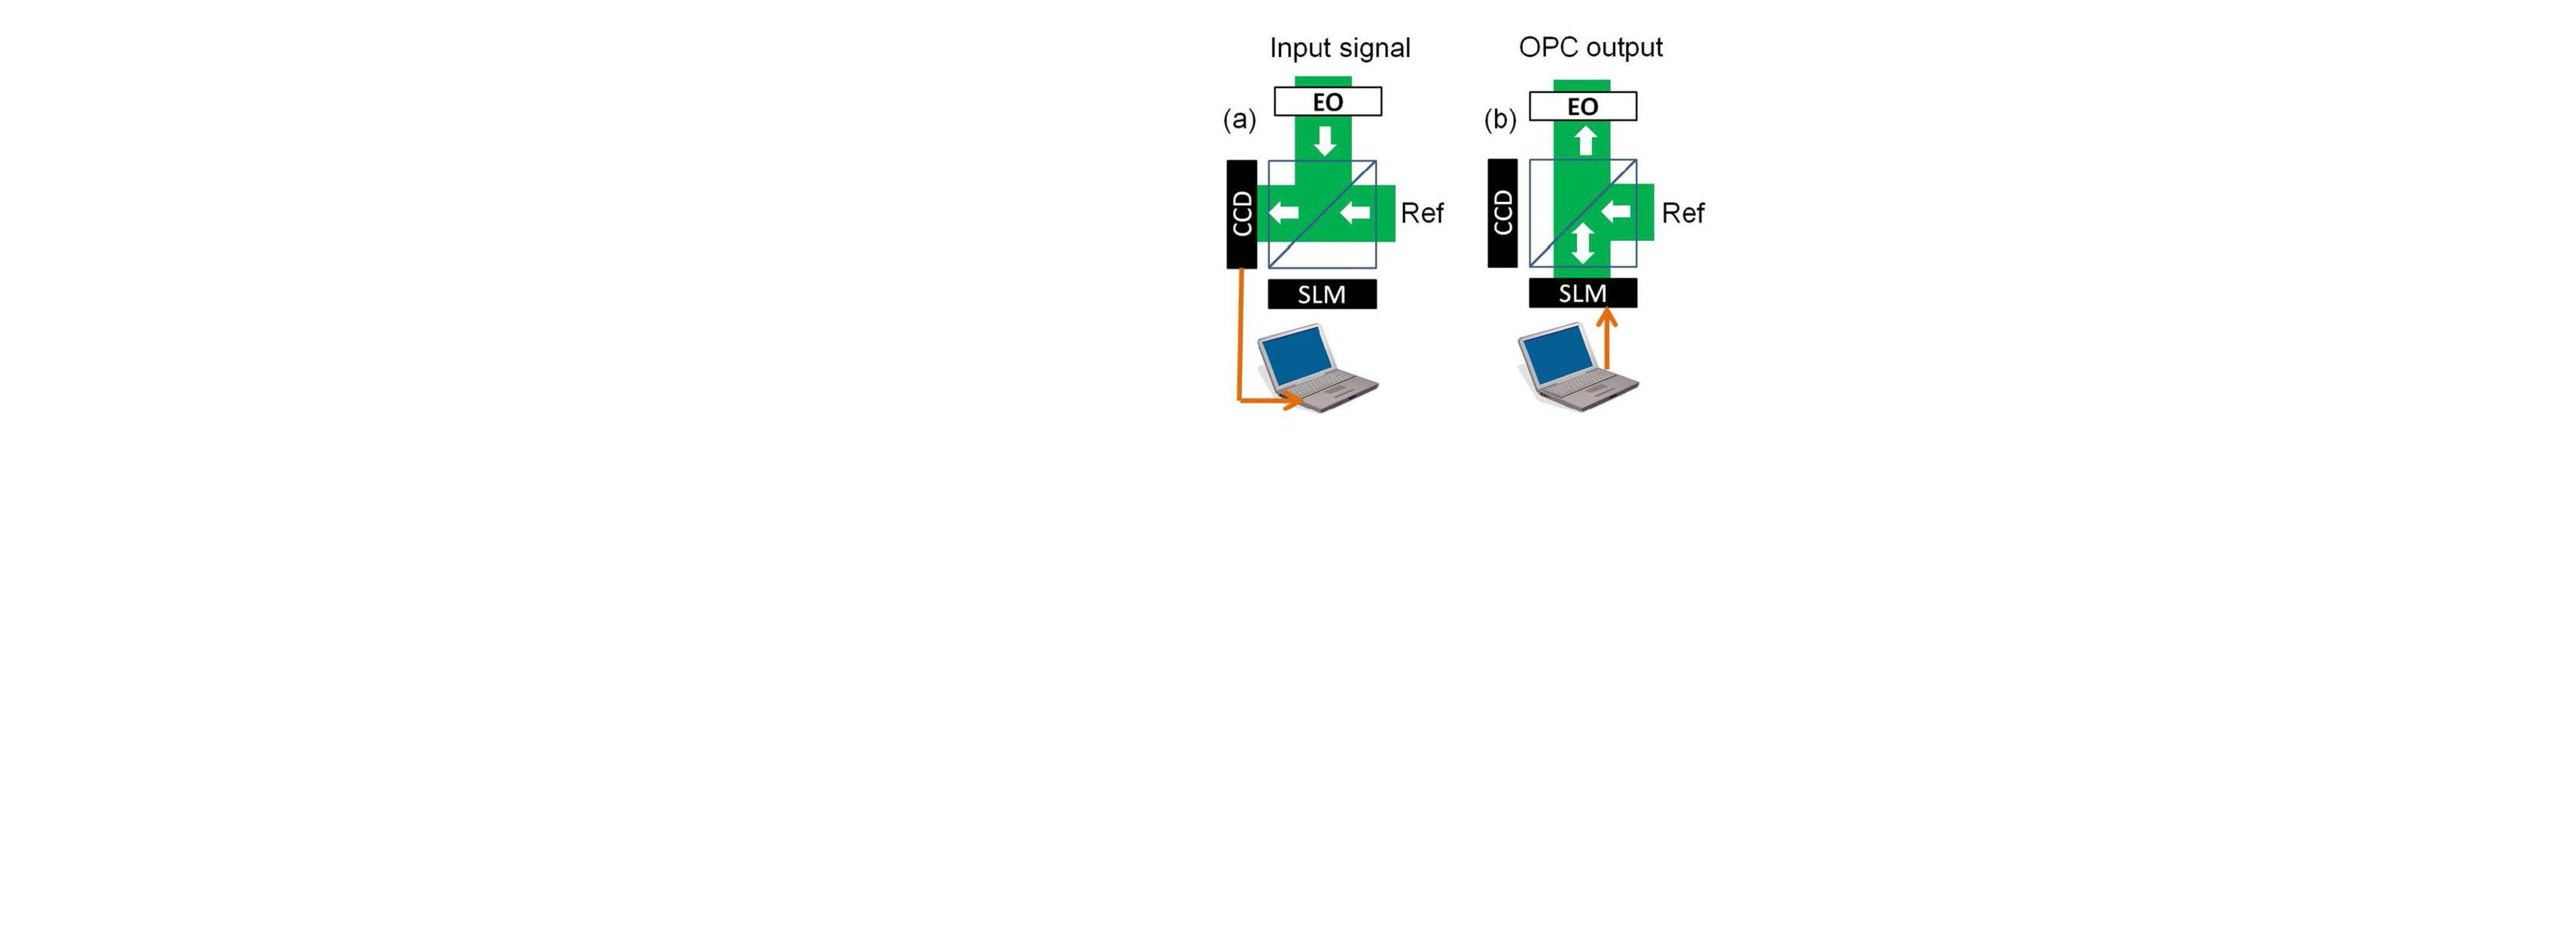
\includegraphics[scale=0.7]{Figchapter1.1.pdf}
	\caption{数字光学相位共轭示意图}
	\label{fig:Schematic_of_digital_optical_phase_conjugation}
\end{figure}

由于SLM和DMD等元件的出现,使数字光学相位共轭调制变成可能,数字光学相位共轭技术的工作原理如图\ref{fig:Schematic_of_digital_optical_phase_conjugation}所示。在获得输出场的光场信息后,利用数字元器件产生相位共轭光,进而实现透过散射介质的聚焦和成像。2008年,Z. Yaqoob等人首次提出了一种基于光学相位共轭的散射成像模型,通过单次记录光场信息克服介质的散射实现成像。2009年,Pauriss等人利用了数字光学相位共轭技术实现了对光纤输出光场的控制和补偿。随后,数字光学相位共轭技术被应用于透过散射介质和多模光纤聚焦。

数字光学相位共轭技术虽然在调制效率方面具有劣势,但是对于透过复杂介质成像方面的应用有着得天独厚的优势。数字光学相位共轭技术利用计算机记录其输出光场分布,利用调制器生成共轭光,可以对无数个输入光场进行重构,相较而言,非线性光学相位共轭技术不具备此特点。在未来发展中,如何提高数字光学相位共轭技术的效率问题,将决定数字光学相位共轭技术在未来应用中的地位。

\subsection{基于反馈优化波前整形的散射介质成像技术}

基于反馈优化的波前整形技术利用优化算法(非线性或线性),通过迭代获取到目标光场所对应的最优波前,从而实现透过散射介质聚焦或成像。本质上,基于反馈优化的波前整形技术将散射介质对于光场的调制过程看作“黑箱”处理,通过迭代算法获取相应的波前,进而实现了对于输出光场的模式以及不同模式之间耦合的控制。

2007年,A. P. Mosk课题组利用SLM对入射到随机散射介质中的光波进行波前相位调制,采用反馈控制算法对空间光调制器的SLM像素进行逐个优化,通过不断迭代的方式获取最优波前,所得的最优波前幅值或相位可以适当补偿由介质散射引起的波前畸变,最终得到了亮度高于调制前散斑1000倍的聚焦光斑,远远优于光学透镜的聚焦效果,实验装置和实验结果分别如图2和图3所示。

